% Sections/section2.tex

% Slide Mục lục (Highlight phần 2)
\begin{frame}{Contents}
    \Large
    \vspace{-0.5cm} 
    
    \begin{enumerate}
        \setlength{\itemsep}{0.4cm} 
        
        \item \textcolor{gray}{Introduction to Database Security Issues}
        
        \item \textbf{Discretionary Access Control (DAC)}
        
        \item Mandatory Access Control (MAC)
        \item Role-Based Access Control (RBAC)
        \item Attribute-Based Access Control (ABAC)
        \item Context-Based Access Control (CBAC)
        
    \end{enumerate}
\end{frame}

% --- SỬA LỖI NGẮT DÒNG Ở ĐÂY ---
% Thêm dấu \\ để ép xuống dòng sau chữ Discretionary
\section{Discretionary \\ Access Control (DAC)}


% Slide nội dung đầu tiên của Section 2
\begin{frame}{Discretionary Access Control (DAC)}
    \Large % Cỡ chữ chủ đạo
    
    \begin{itemize}
        \vspace{-1.5cm} % Kéo nội dung lên cao
        
        % Nhóm ý 1: Quyền của Owner
        \item User can protect what they own.
        \item Owner may grant access to other.
        \item Owner can define the type of access (read/write/execute/...) given to others.
        
        \vspace{0.6cm} % Tách biệt rõ ràng với ý dưới
        
        % Nhóm ý 2: Cách thực thi (Có in đậm từ khóa)
        \item The typical method of enforcing \textbf{discretionary access control} in a database system is based on the \textbf{granting} and \textbf{revoking privileges}.
        
    \end{itemize}
\end{frame}


% Slide tiếp theo trong Sections/section2.tex

\begin{frame}{Types of Discretionary Privileges (1)}
    \Large % Cỡ chữ chủ đạo
    
    \begin{itemize}
        \vspace{-1.5cm} % Kéo nội dung lên cao
        
        % Ý chính 1
        \item The \textbf{account level}:
        
        \begin{itemize}
            \large % Cỡ chữ ý phụ
            \setlength{\itemsep}{0.2cm}
            
            % Sub-item (Tự động có dấu tròn rỗng)
            \item At this level, the DBA specifies the particular privileges that each account holds independently of the relations in the database.
        \end{itemize}
        
        \vspace{0.5cm} % Tạo khoảng cách giữa 2 phần cho thoáng
        
        % Ý chính 2
        \item The \textbf{relation level} (or \textbf{table level}):
        
        \begin{itemize}
            \large 
            \setlength{\itemsep}{0.2cm}
            
            % Sub-item
            \item At this level, the DBA can control the privilege to access each individual relation or view in the database.
        \end{itemize}
        
    \end{itemize}
\end{frame}


% Slide tiếp theo trong Sections/section2.tex

\begin{frame}{Types of Discretionary Privileges (2)}
    \Large % Cỡ chữ chủ đạo
    
    \begin{itemize}
        \vspace{-0.5cm} % Kéo nội dung lên cao
        
        % Ý chính
        \item The privileges at the \textbf{account level} apply to the capabilities provided to the account itself and can include:
        
        \begin{itemize}
            \large % Cỡ chữ Level 2
            \setlength{\itemsep}{0.1cm} % Chỉnh khoảng cách nhỏ lại (0.1cm) để nhét vừa 6 dòng
            
            % Các mục con (Tự động có dấu tròn rỗng)
            \item the \textbf{CREATE SCHEMA} or \textbf{CREATE TABLE} privilege, to create a schema or base relation;
            
            \item the \textbf{CREATE VIEW} privilege;
            
            \item the \textbf{ALTER} privilege, to apply schema changes such adding or removing attributes from relations;
            
            \item the \textbf{DROP} privilege, to delete relations or views;
            
            \item the \textbf{MODIFY} privilege, to insert, delete, or update tuples;
            
            \item and the \textbf{SELECT} privilege, to retrieve information from the database by using a \textbf{SELECT} query.
        \end{itemize}
        
    \end{itemize}
\end{frame}

% Slide tiếp theo trong Sections/section2.tex

\begin{frame}{Types of Discretionary Privileges (3)}
    \Large % Cỡ chữ chủ đạo
    
    \begin{itemize}
        \vspace{-0.5cm} % Kéo nội dung lên cao
        
        % Ý chính 1
        \item The second level of privileges applies to the \textbf{relation level}
        
        \begin{itemize}
            \large
            \setlength{\itemsep}{0.1cm}
            \item This includes \textbf{base relations} and virtual (\textbf{view}) relations.
        \end{itemize}
        
        \vspace{0.2cm} % Khoảng cách nhỏ
        
        % Ý chính 2
        \item In SQL the following types of privileges can be granted on each individual relation R:
        
        \begin{itemize}
            \large % Cỡ chữ Level 2
            \setlength{\itemsep}{0.2cm}
            
            % Mục con 1: SELECT
            \item \textbf{SELECT} (retrieval or read) privilege on R:
            
            % Level 3: Giải thích chi tiết
            \begin{itemize}
                \normalsize % Cỡ chữ nhỏ hơn chút
                \setlength{\itemsep}{0.1cm}
                \item This gives the account retrieval privilege.
                \item The \textbf{SELECT} statement is used to retrieve tuples from R.
            \end{itemize}
            
            % Mục con 2: REFERENCES
            \item \textbf{REFERENCES} privilege on R:
            
            % Level 3: Giải thích chi tiết
            \begin{itemize}
                \normalsize 
                \setlength{\itemsep}{0.1cm}
                \item This gives the account the capability to \textbf{reference} relation R when specifying integrity constraints.
                \item The privilege can also be \textbf{restricted} to specific attributes of R.
            \end{itemize}
            
        \end{itemize}
        
    \end{itemize}
\end{frame}


% Slide tiếp theo trong Sections/section2.tex

\begin{frame}{Types of Discretionary Privileges (4)}
    \Large % Cỡ chữ chủ đạo
    
    \begin{itemize}
        \vspace{-0.5cm} % Kéo nội dung lên cao
        
        % Ý chính 1
        \item In SQL the following types of privileges can be granted on each individual relation R (contd.):
        
        \begin{itemize}
            \large % Cỡ chữ Level 2
            \setlength{\itemsep}{0.2cm}
            
            % Mục con: MODIFY
            \item \textbf{MODIFY} privileges on R:
            
            % Level 3: Giải thích chi tiết
            \begin{itemize}
                \normalsize % Cỡ chữ nhỏ hơn chút
                \setlength{\itemsep}{0.1cm}
                
                \item This gives the account the capability to modify tuples of R.
                
                \item In SQL this privilege is further divided into \textbf{UPDATE}, \textbf{DELETE}, and \textbf{INSERT} privileges to apply the corresponding SQL command to R.
                
                \item In addition, both the \textbf{INSERT} and \textbf{UPDATE} privileges can specify that only certain attributes can be updated by the account.
            \end{itemize}
            
        \end{itemize}
        
        \vspace{0.4cm} % Khoảng cách thoáng trước ý chính cuối
        
        % Ý chính 2
        \item Notice that to create a \textbf{view}, the account must have \textbf{SELECT} privilege on all relations involved in the view definition.
        
    \end{itemize}
\end{frame}

% Slide tiếp theo trong Sections/section2.tex

\begin{frame}{Types of Discretionary Privileges (5)}
    \Large % Cỡ chữ chủ đạo
    
    \begin{itemize}
        \vspace{-1.5cm} % Kéo nội dung lên cao
        
        % Ý chính
        \item The granting and revoking of privileges generally follow an authorization model for discretionary privileges known as the access matrix model where:
        
        \begin{itemize}
            \large % Cỡ chữ Level 2
            \setlength{\itemsep}{0.3cm} % Tăng giãn dòng lên 0.3cm cho thoáng vì mỗi ý khá dài
            
            % Sub-item 1: Rows
            \item The \textbf{rows} of a matrix M represents \textbf{subjects} (users, accounts, programs)
            
            % Sub-item 2: Columns
            \item The \textbf{columns} represent \textbf{objects} (relations, records, columns, views, operations).
            
            % Sub-item 3: Position M(i,j)
            \item Each position \textbf{M(i,j)} in the matrix represents the types of privileges (read, write, update) that \textbf{subject i} holds on \textbf{object j}.
        \end{itemize}
        
    \end{itemize}
\end{frame}

% --- Slide: Access matrix model ---
\begin{frame}[plain]
    \begin{columns}
        % Cột trái: Chữ to bự
        \begin{column}{0.35\textwidth}
            \vspace{2cm} % Đẩy chữ xuống một chút cho cân đối với bảng
            \Huge \textbf{Access \\[0.3cm] matrix \\[0.3cm] model}
        \end{column}
        
        % Cột phải: Chèn hình ảnh bảng Access Matrix
        \begin{column}{0.65\textwidth}
            \centering
            % Bạn nhớ đổi "access_matrix.jpg" thành đúng tên file ảnh của bạn nhé!
            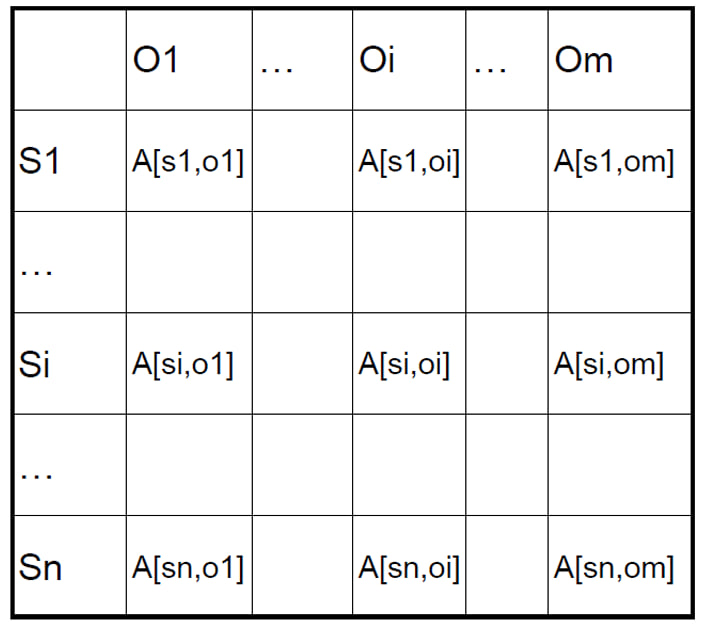
\includegraphics[width=\textwidth]{Assets/accessmatrix.jpg}
        \end{column}
    \end{columns}
\end{frame}

% Slide tiếp theo trong Sections/section2.tex

\begin{frame}{Types of Discretionary Privileges (6)}
    \Large % Cỡ chữ chủ đạo
    
    \begin{itemize}
        \vspace{-1.5cm} % Kéo nội dung lên cao
        
        % Ý chính
        \item To control the granting and revoking of relation privileges, for each relation R in a database:
        
        \begin{itemize}
            \large % Cỡ chữ Level 2
            \setlength{\itemsep}{0.3cm} % Giãn dòng cho thoáng
            
            % Sub-item 1
            \item The owner of a relation is given \textbf{all} privileges on that relation.
            
            % Sub-item 2: Có chữ màu xanh dương (pass privileges)
            \item The owner account holder can \textbf{\textcolor{blue}{pass privileges}} on any of the owned relation to other users by \textbf{granting} privileges to their accounts.
            
            % Sub-item 3: Có chữ màu xanh dương (take back)
            \item The owner account holder can also \textbf{\textcolor{blue}{take back}} the \textbf{privileges} by \textbf{revoking} privileges from their accounts.
        \end{itemize}
        
    \end{itemize}
\end{frame}

% Slide tiếp theo trong Sections/section2.tex

\begin{frame}{Specifying Privileges Using Views}
    \Large % Cỡ chữ chủ đạo
    
    \begin{itemize}
        \vspace{-1.5cm} % Kéo nội dung lên cao
        
        % Ý chính
        \item The mechanism of \textbf{views} is an important discretionary authorization mechanism in its own right.
        
        \begin{itemize}
            \large % Cỡ chữ Level 2
            \setlength{\itemsep}{0.3cm} % Giãn dòng thoáng
            
            % Sub-item 1
            \item If the owner A of a relation R wants another account B to be able to \textbf{\textcolor{blue}{retrieve only some fields}} of R, then A can \textbf{\textcolor{blue}{create a view}} V of R that includes \textbf{\textcolor{blue}{only those attributes}} and then grant SELECT on V to B.
            
            % Sub-item 2
            \item The same applies to limiting B to retrieving \textbf{\textcolor{blue}{only certain tuples of}} R; a view V' can be created by defining the view by means of a query that selects only those tuples from R that A wants to allow B to access.
        \end{itemize}
        
    \end{itemize}
\end{frame}

% Slide tiếp theo trong Sections/section2.tex

\begin{frame}{Revoking Privileges}
    \Large % Cỡ chữ chủ đạo
    
    \begin{itemize}
        \vspace{-1.5cm} % Kéo nội dung lên cao
        
        % Ý chính
        \item In some cases it is desirable to grant a privilege to a user temporarily.
        
        \begin{itemize}
            \large % Cỡ chữ Level 2
            \setlength{\itemsep}{0.3cm} % Giãn dòng thoáng cho dễ đọc
            
            % Sub-item 1
            \item The owner of a relation may want to grant the \textbf{SELECT} privilege to a user for a specific task and then revoke that privilege once the task is completed.
            
            % Sub-item 2
            \item Hence, a mechanism for \textbf{revoking} privileges is needed. In SQL, a \textbf{REVOKE} command is included for the purpose of \textbf{canceling privileges}.
        \end{itemize}
        
    \end{itemize}
\end{frame}

% Slide tiếp theo trong Sections/section2.tex

\begin{frame}{Propagation of Privileges using the GRANT OPTION}
    \Large % Cỡ chữ chủ đạo
    
    \begin{itemize}
        \vspace{-0.5cm} % Kéo nội dung lên cao
        
        % Ý chính 1
        \item Whenever the owner A of a relation R grants a privilege on R to another account B, privilege can be given to B with or without the \textbf{GRANT OPTION}.
        
        \vspace{0.2cm} % Khoảng cách nhỏ
        
        % Ý chính 2
        \item If the \textbf{GRANT OPTION} is given, this means that B can also grant that privilege on R to other accounts.
        
        \begin{itemize}
            \normalsize % Cỡ chữ Level 2
            \setlength{\itemsep}{0.2cm} % Giãn dòng vừa phải
            
            % Sub-item 1
            \item Suppose that B is given the \textbf{GRANT OPTION} by A and that B then grants the privilege on R to a third account C, also with \textbf{GRANT OPTION}. In this way, privileges on R can \textbf{propagate} to other accounts without the knowledge of the owner of R.
            
            % Sub-item 2: Có màu xanh dương
            \item If the owner account \textbf{A now revokes} the privilege granted to B, \textbf{\textcolor{blue}{all the privileges that B propagated}} based on that privilege should automatically \textbf{\textcolor{blue}{be revoked}} by the system.
        \end{itemize}
        
    \end{itemize}
\end{frame}


% Slide sơ đồ cây
\begin{frame}{Limiting the horizontal propagation}
    \centering 
    % Bỏ dấu trừ đi, cho nó nhích xuống một xíu cho thoáng
    \vspace{0.2cm} 
    
    % Thu nhỏ toàn bộ sơ đồ còn 85% chiều rộng slide
    \resizebox{0.55\textwidth}{!}{
    \begin{tikzpicture}[
        % --- CẤU HÌNH CHUNG ---
        node distance=2.0cm and 1.5cm, 
        accountbox/.style={
            rectangle, draw=black, thick, fill=cyan!10, 
            minimum width=1.8cm, minimum height=0.8cm, 
            align=center, font=\bfseries\large 
        },
        connarrow/.style={
            ->, >=Stealth, ultra thick 
        },
        labeltext/.style={
            font=\normalsize, align=left 
        }
    ]
        
        % --- VẼ CÁC HỘP (NODES) ---
        \node[accountbox] (a1) {A1};
        \node[accountbox, below=of a1] (a2) {A2};
        \node[accountbox, below left=of a2] (a3) {A3};
        \node[accountbox, below right=of a2] (a4) {A4};
        
        % --- VẼ CÁC MŨI TÊN KẾT NỐI ---
        \draw[connarrow] (a1) -- (a2) 
            node[midway, right=0.5cm, labeltext] {Grant with\\horizontal propagation\\$i=2$};
            
        \draw[connarrow] (a2) -- (a3)
            node[midway, above left=-0.2cm, labeltext] {Grant};
            
        \draw[connarrow] (a2) -- (a4)
            node[midway, above right=-0.2cm, labeltext] {Grant};
            
        % --- VẼ MŨI TÊN NÉT ĐỨT Ở DƯỚI ---
        \draw[dashed, ->, ultra thick] 
            ($(a3.south) + (0,-0.8cm)$) -- ($(a4.south) + (0,-0.8cm)$)
            node[midway, below] {\large $i=2$};

    \end{tikzpicture}
    } % Kết thúc resizebox
\end{frame}

% --- Slide: Limiting the vertical propagation ---
\begin{frame}{Limiting the vertical propagation}
    \centering 
    \vspace{-0.3cm} % Cân đối lại khoảng cách trên dưới
    \resizebox{0.65\textwidth}{!}{
    \begin{tikzpicture}[
        % Bê nguyên style cực chuẩn của bạn xuống đây
        accountbox/.style={
            rectangle, draw=black, thick, fill=cyan!10, 
            minimum width=1.8cm, minimum height=0.8cm, 
            align=center, font=\bfseries\large 
        },
        connarrow/.style={
            ->, >=Stealth, ultra thick 
        },
        labeltext/.style={
            font=\normalsize, align=center % Đổi thành align=center cho chữ nằm giữa đẹp hơn
        }
    ]
        
        % --- VẼ CÁC HỘP (NODES) THEO TỌA ĐỘ ---
        \node[accountbox] (a1) at (0, 0) {A1};
        \node[accountbox] (a2) at (0, -2.2) {A2};
        \node[accountbox] (a3) at (-2.5, -4.5) {A3};
        \node[accountbox] (a4) at (2.5, -4.5) {A4};
        \node[accountbox] (a5) at (-4, -6.8) {A5};
        \node[accountbox] (a6) at (-1, -6.8) {A6};
        
        % --- VẼ CÁC MŨI TÊN KẾT NỐI ---
        \draw[connarrow] (a1) -- (a2) 
            node[midway, right=0.3cm, labeltext] {Grant with\\vertical propagation\\$j=2$};
            
        \draw[connarrow] (a2) -- (a3) 
            node[midway, above left=-0.1cm and 0.1cm, labeltext] {Grant\\with $j=1$};
            
        \draw[connarrow] (a2) -- (a4) 
            node[midway, above right=-0.1cm and 0.1cm, labeltext] {Grant\\with $j=0$};
            
        \draw[connarrow] (a3) -- (a5) 
            node[midway, above left=-0.1cm and 0.1cm, labeltext] {Grant\\with $j=0$};
            
        \draw[connarrow] (a3) -- (a6) 
            node[midway, above right=-0.1cm and 0.1cm, labeltext] {Grant\\with $j=0$};
            
        % --- VẼ MŨI TÊN NÉT ĐỨT Ở BÊN PHẢI ---
        % Mũi tên kéo dài từ mức A2 xuống mức A6
        \draw[dashed, ->, >=Stealth, ultra thick] (4.5, -1) -- (4.5, -6.8) 
            node[right=0.2cm, font=\large] {$j=2$};

    \end{tikzpicture}
    }
\end{frame}
% Slide tiếp theo trong Sections/section2.tex

\begin{frame}{An Example (1)}
    \Large % Cỡ chữ chủ đạo
    
    \begin{itemize}
        \vspace{-0.5 cm} % Kéo nội dung lên cao
        
        % Ý chính 1
        \item Suppose that the DBA creates four accounts:
        \begin{itemize}
            \large
            \item A1, A2, A3, A4
        \end{itemize}
        
        % Ý chính 2
        \item and wants only A1 to be able to create base relations. Then the DBA must issue the following GRANT command in SQL:
        
        \vspace{0.3cm} % Tách dòng lệnh SQL ra
        % Dòng lệnh SQL 1: GRANT (đậm) + code (máy đánh chữ)
        {\normalsize \textbf{GRANT} \texttt{CREATETAB TO A1;}}
        \vspace{0.3cm}
        
        % Ý chính 3
        \item In SQL2 the same effect can be accomplished by having the DBA issue a \textbf{CREATE SCHEMA} command as follows:
        
        \vspace{0.3cm}
        % Dòng lệnh SQL 2: Màu đỏ nâu + Đậm + Code
        % Mình dùng mã màu red!70!black để tạo màu đỏ sẫm giống ảnh
        {\normalsize \textcolor{red!70!black}{\textbf{CREATE SCHEMA} \texttt{EXAMPLE} \textbf{AUTHORIZATION} \texttt{A1;}}}
        
    \end{itemize}
\end{frame}


% Slide tiếp theo trong Sections/section2.tex

\begin{frame}{An Example (2)}
    \Large % Cỡ chữ chủ đạo
    
    \begin{itemize}
        \vspace{-0.5cm} % Kéo nội dung lên cao
        
        % Ý chính 1
        \item User account \textbf{A1 can create tables} under the schema called \textbf{\textit{EXAMPLE}}.
        
        % Ý chính 2
        \item Suppose that A1 \textbf{creates} the two base relations \textbf{EMPLOYEE} and \textbf{DEPARTMENT}:
        
        \begin{itemize}
            \normalsize
            \setlength{\itemsep}{0.2cm}
            % Sub-item: Có chữ màu xanh dương
            \item A1 is then \textbf{owner} of these two relations and hence \textcolor{blue}{\textbf{all the relation privileges}} on each of them.
        \end{itemize}
        
        % Ý chính 3
        \item Suppose that A1 wants to grant A2 the privilege to insert and delete tuples in both of these relations, but A1 does not want A2 to be able to propagate these privileges to additional accounts:
        
        \vspace{0.3cm} % Tách dòng lệnh SQL ra
        
        % Dòng lệnh SQL: Màu đỏ nâu, chia làm 2 dòng
        {
            \normalsize \color{red!70!black} % Thiết lập màu đỏ nâu cho cả khối
            \textbf{GRANT INSERT}, \textbf{DELETE ON} \\[0.1cm] % Dòng 1
            \hspace{1.5cm} \texttt{EMPLOYEE}, \texttt{DEPARTMENT} \textbf{TO} \texttt{A2}; % Dòng 2 (thụt đầu dòng)
        }
        
    \end{itemize}
\end{frame}




% Slide tiếp theo trong Sections/section2.tex
% Slide An Example (3) - Vẽ lại Schema Database
\begin{frame}{An Example (3)}
    \Large % Cỡ chữ lớn
    \vspace{-0.5cm} % Kéo lên xíu
    
    \begin{columns}[T] % Căn lề trên (Top) cho 2 cột
        
        % --- CỘT TRÁI: CHỨA CÁC BẢNG (SCHEMAS) ---
        \begin{column}{0.65\textwidth}
        
            % Bảng 1: EMPLOYEE
            \textbf{EMPLOYEE} \\
            \vspace{0.1cm}
            % Dùng resizebox để bảng tự co giãn vừa chiều ngang cột
            \resizebox{\textwidth}{!}{ 
                \begin{tabular}{|c|c|c|c|c|c|c|}
                    \hline
                    % Tô màu nền xám nhạt cho hàng tiêu đề
                    \rowcolor{gray!20} 
                    Name & \underline{Ssn} & Bdate & Address & Sex & Salary & Dno \\
                    \hline
                \end{tabular}
            }
            
            \vspace{0.8cm} % Khoảng cách giữa 2 bảng
            
            % Bảng 2: DEPARTMENT
            \textbf{DEPARTMENT} \\
            \vspace{0.1cm}
            \resizebox{0.75\textwidth}{!}{ 
                \begin{tabular}{|c|c|c|}
                    \hline
                    \rowcolor{gray!20}
                    \underline{Dnumber} & Dname & Mgr\_ssn \\
                    \hline
                \end{tabular}
            }
            
        \end{column}
        
        % --- CỘT PHẢI: CHÚ THÍCH (FIGURE CAPTION) ---
        \begin{column}{0.35\textwidth}
            \large
            \vspace{2cm} % Đẩy text xuống giữa cho cân đối với hình bên trái
            
            \textbf{Figure 24.1} \\
            Schemas for the two relations EMPLOYEE and DEPARTMENT.
        \end{column}
        
    \end{columns}
\end{frame}

% Slide tiếp theo trong Sections/section2.tex

\begin{frame}{An Example (4)}
    \large % Cỡ chữ chủ đạo
    
    \begin{itemize}
        \vspace{-0.5cm} % Kéo nội dung lên cao
        
        % Ý chính 1
        \item Suppose that A1 wants to allow A3 to retrieve information from either of the two tables and also to be able to propagate the SELECT privilege to other accounts.
        
        % Ý chính 2
        \item A1 can issue the command:
        
        \vspace{0.2cm}
        % Dòng lệnh SQL 1: Màu đỏ nâu, ngắt 2 dòng
        {
            \normalsize \color{red!70!black}
            \textbf{GRANT SELECT ON} \texttt{EMPLOYEE}, \texttt{DEPARTMENT} \\[0.1cm]
            \hspace{1.5cm} \textbf{TO} \texttt{A3} \textbf{WITH GRANT OPTION};
        }
        \vspace{0.2cm}
        
        % Ý chính 3
        \item A3 can grant the \textbf{SELECT} privilege on the \textbf{EMPLOYEE} relation to A4 by issuing:
        
        \vspace{0.2cm}
        % Dòng lệnh SQL 2
        {
            \normalsize \color{red!70!black}
            \textbf{GRANT SELECT ON} \texttt{EMPLOYEE} \textbf{TO} \texttt{A4};
        }
        
        % Ý phụ (Sub-item)
        \begin{itemize}
            \large
            \item Notice that A4 can't propagate the SELECT privilege because GRANT OPTION was not given to A4.
        \end{itemize}
        
    \end{itemize}
\end{frame}

% Slide tiếp theo trong Sections/section2.tex

\begin{frame}{An Example (5)}
    \Large % Cỡ chữ chủ đạo
    
    \begin{itemize}
        \vspace{-1.5cm} % Kéo nội dung lên cao
        
        % Ý chính 1
        \item Suppose that A1 decides to revoke the SELECT privilege on the EMPLOYEE relation from A3; A1 can issue:
        
        \vspace{0.2cm}
        % Dòng lệnh SQL: Màu đỏ nâu
        {
            \normalsize \color{red!70!black}
            \textbf{REVOKE SELECT ON} \texttt{EMPLOYEE} \textbf{FROM} \texttt{A3};
        }
        \vspace{0.2cm}
        
        % Ý chính 2
        \item The DBMS must now \textbf{automatically revoke the SELECT privilege on EMPLOYEE from A4}, too, because A3 granted that privilege to A4 and A3 does not have the privilege any more.
        
    \end{itemize}
\end{frame}

% --- Slide 39: An Example (6) ---
\begin{frame}{An Example (6)}
    \Large
    \begin{itemize}
        \vspace{-0.5cm}
        \item Suppose that A1 wants to give back to A3 a limited capability to SELECT from the EMPLOYEE relation and wants to allow A3 to be able to propagate the privilege.
        \begin{itemize}
            \large
            \item The limitation is to retrieve only the NAME, BDATE, and ADDRESS attributes and only for the tuples with DNO=5.
        \end{itemize}
        
        \item A1 then create the view:
        \vspace{0.1cm}
        {
            \normalsize
            \textbf{CREATE VIEW} \texttt{A3\_EMPLOYEE} \textbf{AS} \\
            \hspace{0.5cm} \textbf{SELECT} \texttt{NAME, BDATE, ADDRESS} \\
            \hspace{0.5cm} \textbf{FROM} \texttt{EMPLOYEE} \textbf{WHERE} \texttt{DNO = 5;}
        }
        \vspace{0.1cm}
        
        \item After the view is created, A1 can grant \textbf{SELECT} on the view \textit{A3\_EMPLOYEE} to A3 as follows:
        \vspace{0.1cm}
        {
            \normalsize \color{red!70!black}
            \textbf{GRANT SELECT ON} \texttt{A3\_EMPLOYEE} \textbf{TO} \texttt{A3} \\
            \textbf{WITH GRANT OPTION;}
        }
    \end{itemize}
\end{frame}

% --- Slide 40: An Example (7) ---
\begin{frame}{An Example (7)}
    \Large
    \begin{itemize}
        \vspace{-1.5cm}
        \item Finally, suppose that A1 wants to allow A4 to update only the SALARY attribute of EMPLOYEE;
        \item A1 can issue:
        
        \vspace{0.2cm}
        {
            \normalsize \color{red!70!black}
            \textbf{GRANT UPDATE ON} \texttt{EMPLOYEE (SALARY)} \textbf{TO} \texttt{A4;}
        }
        \vspace{0.2cm}
        
        \item The \textbf{UPDATE} or \textbf{INSERT} privilege can specify particular attributes that may be updated or inserted in a relation.
        
        \item Other privileges (\textbf{SELECT}, \textbf{DELETE}) are not attribute specific.
    \end{itemize}
\end{frame}

% --- Slide 41: Inherent weakness of DAC ---
\begin{frame}{Inherent weakness of DAC}
    \Large
    \begin{itemize}
        \vspace{-1.5cm}
        \item \textbf{Unrestricted DAC} allows information from an object which can be read by a subject to be written to any other object.
        
        \begin{itemize}
            \large
            \item Bob is denied access to file Y, so he asks Alice to copy Y to X that he can access.
        \end{itemize}
        
        \item Suppose our users are trusted not to do this deliberately.
        
        \item It is still possible for \textbf{Trojan Horses} to copy information from one object to another.
    \end{itemize}
\end{frame}

% Định nghĩa chung cho hình vẽ Trojan Horse (đỡ phải viết lại nhiều lần)
\tikzset{
    user/.style={circle, draw=black, thick, minimum size=1.2cm, align=center, fill=white},
    file/.style={rectangle, draw=black, thick, minimum width=2cm, minimum height=1.2cm, align=center, fill=white},
    program/.style={rectangle, draw=black, thick, minimum width=1.5cm, minimum height=2cm, align=center, fill=gray!10},
    th/.style={rectangle, draw=black, thick, fill=white, minimum size=0.5cm},
    arrow/.style={->, >=stealth, thick}
}

% --- Slide 42: Trojan horse Example (1) ---
\begin{frame}{Trojan horse Example (1)}
    \centering
    % Thay đổi số 0.9 thành 0.8 hoặc 1.0 tùy thuộc vào việc bạn muốn ảnh to hay nhỏ nhé
    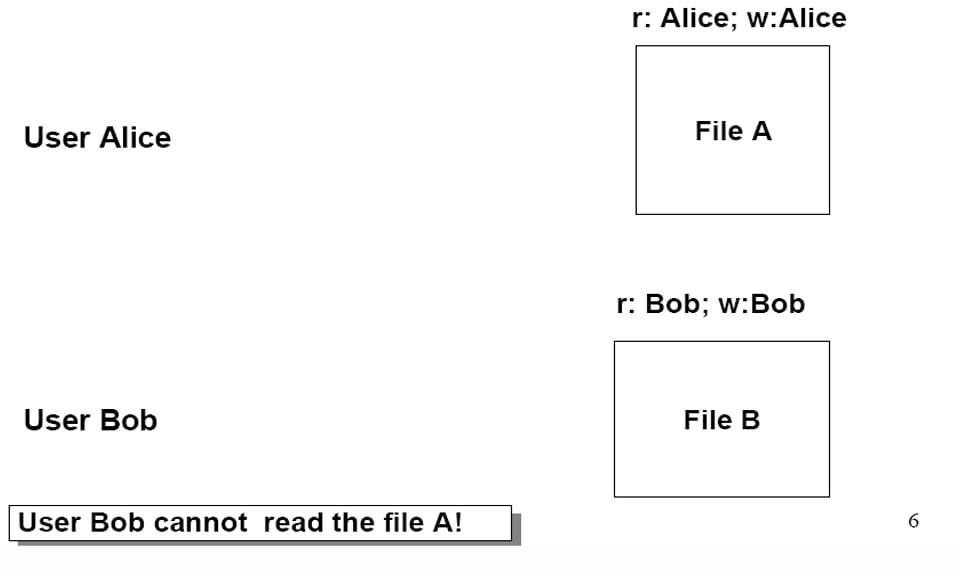
\includegraphics[width=0.9\textwidth]{Assets/trojanhorse1.jpg}
\end{frame}
% --- Slide 43: Trojan horse Example (1) ---
\begin{frame}{Trojan horse Example (2)}
    \centering
    % Thay đổi số 0.9 thành 0.8 hoặc 1.0 tùy thuộc vào việc bạn muốn ảnh to hay nhỏ nhé
    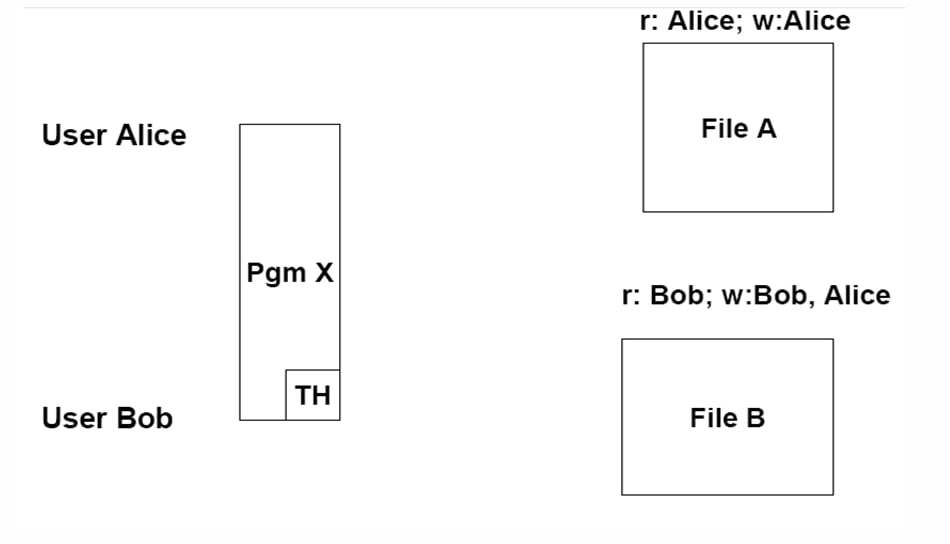
\includegraphics[width=0.9\textwidth]{Assets/trojanhorse2.jpg}
\end{frame}


% --- Slide 44: Trojan horse Example (3) ---

\begin{frame}{Trojan horse Example (3)}
    \centering
    % Thay đổi số 0.9 thành 0.8 hoặc 1.0 tùy thuộc vào việc bạn muốn ảnh to hay nhỏ nhé
    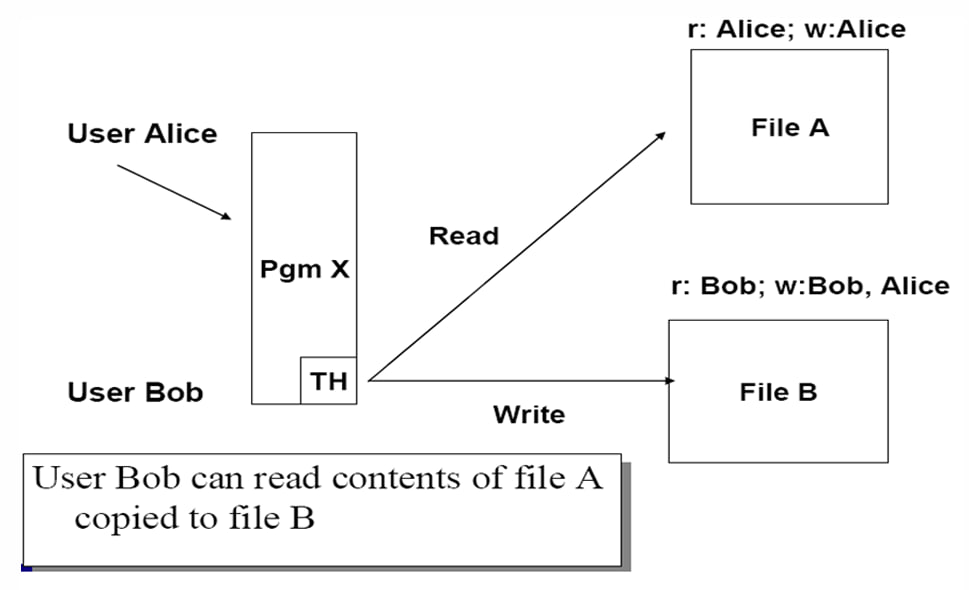
\includegraphics[width=0.8\textwidth]{Assets/trojanhorse3.jpg}
\end{frame}